\documentclass[../projekt.tex]{subfiles}
\begin{document}
%=========================================================================
% (c) Michal Bidlo, Bohuslav Křena, 2008

\section{Úvod}\label{uvod}

Cílem tohoto projektu je návrh a implementace demonstrační aplikace Kargerova
algoritmu pro nalezení minimálního řezu. Daný algoritmus byl navržen a
implementován s využitím vhodných doporučených nástrojů. 

\section{Návrh aplikace}

Předběžný návrh aplikace je důležitým krokem ve vývoji. Při tomto postupu je
možno se vyhnout případným problémům, které by mohly nastat v pozdější
fázi vývoje. Prvním krokem byl návrh základního rozložení hlavního okna aplikace.

	\begin{figure}[ht]
    	\begin{center}
  			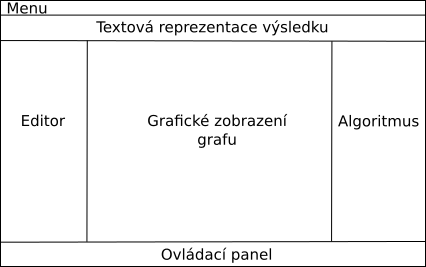
\includegraphics[scale=0.7]{obrazky-figures/layout.png}
  			\caption{Uspořádání hlavního okna aplikace.}
  			\label{fig:layout}
  		\end{center}
	\end{figure}

\subsection{Použité nástroje}

Dalším krokem návrhu aplikace byl výběr programovacího jazyka,
ve kterém bude aplikace napsána. Výsledná aplikace by měla mít grafické
rozhraní (GUI) a měla by být spustitelná na jakékoliv platformě,
především na studentském serveru Merlin. Na základě těchto kritérii byl
zvolen jazyk Java spolu s knihovnou Swing pro tvorbu grafického rozhraní.
Ze seznamu povolených formátů grafů byl vybrán formát mxGraph a knihovna
JGraphX s tímto formátem pracující.

\subsubsection{Swing} 

Swing \cite{swing} je knihovna plně založená na platformě Java a postavená na
AWT (Abstract Windowing Toolkit), sloužící k ovládání počítače pomocí
grafického rozhraní. S využitím této knihovny je možno vytvářet okna (JFrame), 
dialogy (JOptionPane), tlačítka (JButton), seznamy  a mnoho dalšího.


\subsubsection{JGraphX} 

JGraphX \cite{jgraphx} je knihovna licencovaná pod licencí BSD,
založená na Java Swing knihovně, poskytující funkcionalitu
pro vizualizaci a interakci s grafy založenými na systému uzel-hrana.
JGraphX také obsahuje funkce pro podporu XML šablon, různých
importů a exportů a rozvržení grafu.


\section{Implementace}

Hlavní částí vývoje byla implementace algoritmu podle zvolené varianty zadání,
v případě tohoto projektu o Kargerův algoritmus. 

\subsection{Algoritmus}

Jedná se o deterministický randomizovaný algoritmus, který náhodně vybírá hranu
mezi všemi hranami grafu a slučuje koncové uzly této hrany, dokud nezůstanou pouze
dva tzv. super uzly \cite{karger} reprezentující dvě skupiny uzlů v grafu a jedna
hrana/skupina hran představující velikost řezu. Jednoduchý pseudokód hlavní smyčky programu:


\begin{algorithm}
\caption{Karger Algorithm}\label{euclid}
\begin{algorithmic}[1]
\State $Let \; G = (V, E)$
\While {$|V| > 2$}
\State $nahodne \; vyber \; dva \; sousedni \; uzly \; v_1, \; v_2$
\State $mergeCells(v_1, \; v_2)$
%\State $F \gets F\backslash E_{\overline{u}\overline{v}}$
\EndWhile
%\State $Return\, one\, of \,the\, supernodes\, in\, V \,and \,|E_{uv}|$
\end{algorithmic}
\end{algorithm}

\noindent Spojení dvou uzlů: \\

\begin{algorithm}
\caption{$mergeCells(v_1,\; v_2)$}\label{euclid}
\begin{algorithmic}[1]
%\State $x \gets new \, supernode$
%\State {$V(x) \gets V(a) \cup V(b) \; // merge \, the \, vertices$}
\ForEach { $v \in Adj[v_2]$ }
\State $presmeruj \; hranu \; (v,\; v_2) \; na \; (v,\; v_1)$
\State $pripadne \; multihrany \; oznac \; poctem \; hran \; nad \; reprezentujici \; hranou$
%\State $V \ gets (V \backslash \{a,b\}) \ cup \{x\}$
\EndFor
\State $prejmenuj \; v_1 \; // \; konkatenace \; nazvu \; v_1 \; a \; v_2$ 
\State $odstran \; v2 \; a \; vsechny \; jeho \; hrany$ 

\end{algorithmic}
\end{algorithm}

Časová složitost Kargerova algoritmu je polynomiální. Je potřeba vyzkoušet všechny možnosti -- těch je $|E|!$.
Pro každou možnost se spustí jeden běh o $O(|E|)$ krocích, kde každý krok má polynomiální složitost
(zejména kvůli vyhledávání hran ze seznamu při označování multihran a přesměrovávání hran). 

\subsection{Běh aplikace}
Na začátku je uživateli zobrazen výchozí graf. Uživatel může buď spustit krok/běh/algoritmus nad tímto grafem,
nebo tento graf upravit, anebo si vytvořit svůj vlastní graf od základů.

Vnitřně je graf reprezentován třídou \texttt{KargerGraph}, kde je uložen samotný graf a informace o něm.
Důležitými proměnnými jsou \texttt{graphEdges}, kde je seřazený seznam hran, \texttt{curOrder} s aktuálním
pořadím výběru hran v tomto běhu, \texttt{runs} obsahující všechny zatím dosažené výsledky či \texttt{encodedResetGraph},
který uchovává původní graf, který se obnovuje při každém dalším běhu algoritmu.

V každém kroku se nejprve na základě \texttt{curOrder}, čísla kroku a seznamu hran vybere hrana, která se bude odstraňovat a
podle ní se určí na ni napojené uzly, co se spojí. Uvnitř metody \texttt{mergeCells(v1, v2} již probíhá samotné
spojování (tedy přesměrovávání hran, vytváření multihran a odstraňování uzlu \texttt{v2}).

Pokud uživatel zvolí manuální krokování aplikace, je mu v pravém panelu vždy zobrazen řádek algoritmu,
ve kterém se aplikace právě nachází. V první fázi tohoto kroku jsou mu zvýrazněny ty uzly, co se spojí a po dokončení
druhé fáze dostane výsledek po spojení těchto uzlů jako při normálním kroku.

Při dokončení celého běhu algoritmu je kromě původního grafu uživateli zobrazen nejlepší výsledek a ostatní výsledky
jsou seřazeny od nejlepšího pod ním.

\subsection{Struktura aplikace}

Celá aplikace je tvořena jedním hlavním oknem \texttt{MainWindow}. Rozložení hlavního okna
je zobrazeno v návrhu aplikace na obrázku \ref{fig:layout}. Po spuštění aplikace
proběhne načtení a zobrazení výchozího grafu. Uživatel má možnost vybrat pro
zpracování jiný graf. Graf je možno editovat přidáním nebo odebráním uzlů a hran.
Případná komunikace s uživatelem je realizována prostřednictvím dialogových oken. 


	\begin{figure}[ht]
    	\begin{center}
  			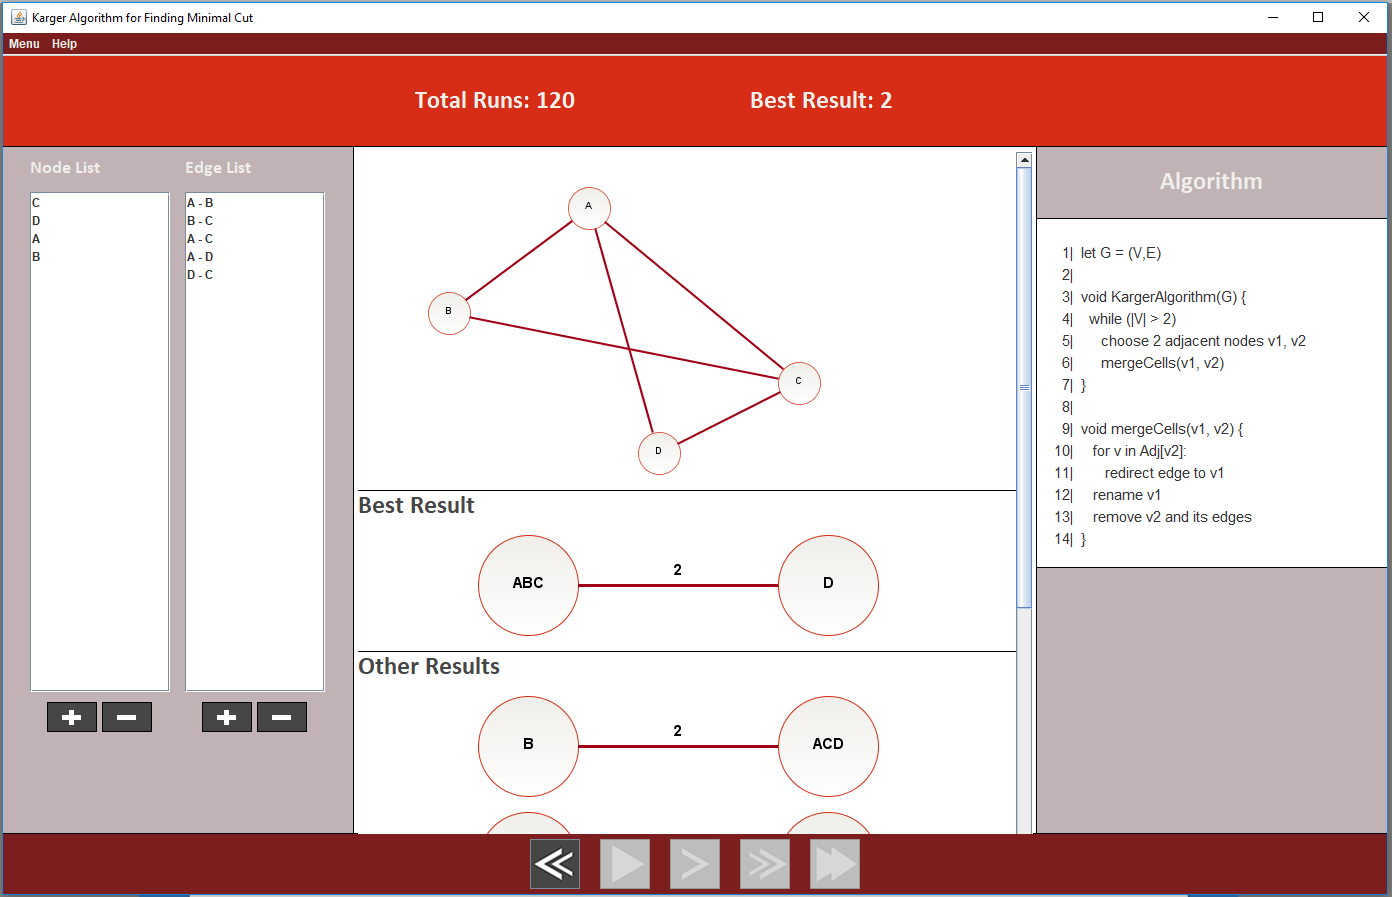
\includegraphics[scale=0.4]{obrazky-figures/finish.png}
  			\caption{Zobrazení výsledku aplikace algoritmu na daný graf.}
  		\end{center}
	\end{figure}


\section{Aplikace}

% seznam minimalnich pozadavku
\subsection{Minimální požadavky}

\begin{itemize}
	\item OpenJDK
	\item Ant (kompilace a spouštění)
	\item JGraphX (knihovna pro práci s grafem)
\end{itemize}

\subsection{Spuštění a instalace}

Odevzdaný archiv obsahuje:

\begin{itemize}
	\item \textit{src} -- adresář se zdrojovými soubory
	\item \textit{lib} -- adresář s využitými knihovnami
	\item \textit{latex} -- zdrovojé kódy této dokumentace 
	\item \textit{README.md}
	\item \textit{dokumentace.pdf} -- tato dokumentace 
	\item \textit{build.xml} - skript pro kompilaci a spuštění aplikace pomocí Ant
\end{itemize}

\noindent Pro sputění aplikace je nutno mít nainstalovaný OpenJDK a Java knihovnu Apache Ant. Aplikace se spouští přes soubor \textit{karger.jar}.


% kratky uvodni popis moznosti aplikace
\subsection{Možnosti aplikace}

\begin{itemize}
	\item vytvoření/načtení/uložení grafu ve formátu XML
	\item editace grafu -- přidání a odebrání uzlu/hrany
	\item ovládání grafu pomocí ovládacího panelu -- resetování, další krok, dokončení jednoho běhu, dokončení algoritmu
	\item podrobnější krokování provádění algoritmu spolu s vyznačením právě provedených částí pseudokódu
	\item přesun uzlů pomocí kliknutí a tažení myší
	\item zobrazení uživatelského manuálu pod záložkou \textit{Help} v horním menu
\end{itemize}



\section{Závěr}

Cílem práce bylo vytvořit aplikaci, která demonstruje Kargerův algoritmus pro
nalezení minimálního řezu. Samotné řešení projektu s využitím knihovny JGraphX
bylo poučné a vedlo k pochopení fungování Kargerova algoritmu. Řešení výsledné
aplikace by mělo uživateli pomoci minimálně s pochopením základního principu algoritmu.

\end{document}
